\documentclass[10pt]{beamer}

\usetheme{Warsaw}
\setbeamertemplate{navigation symbols}{}
\setbeamertemplate{footline}{\insertshorttitle\hfill\insertpagenumber}

\usepackage[utf8]{inputenc}
\usepackage[T1]{fontenc}
\usepackage[french]{babel}

\usepackage{graphicx}
\usepackage{amsmath}
\usepackage{array,multirow,makecell}
\usepackage{xcolor}
\usepackage{hyperref}
\usepackage{listings}


\definecolor{backcolour}{rgb}{0.95,0.95,0.92}
\definecolor{codeblue}{RGB}{33,80,198}
\definecolor{codegreen}{RGB}{0,100,0}
\definecolor{codered}{RGB}{165,0,0}

\lstset{
    backgroundcolor=\color{backcolour},
    basicstyle=\ttfamily\footnotesize,
    commentstyle=\color{codegreen},
    keywordstyle=\color{codeblue},
    stringstyle=\color{codered},
    numbers=left,
    numbersep=4pt,
    breaklines=true,
    tabsize=2
}

\title{Démonstrateur : Arbre Couvrant de Poids Minimal}
\author{Thomas Matthieu \and Tellier Basile}
\date{\today}

\begin{document}

% ========================
\begin{frame}
\titlepage
\end{frame}
% ========================

\begin{frame}{Table des matières}
\tableofcontents
\end{frame}

% ========================
\section{Notions}
% ========================

\begin{frame}{Notions fondamentales}

\begin{itemize}
    \item \textbf{Sommet} : élément de base du graphe
    \item \textbf{Arête} : lien entre deux sommets
    \item \textbf{Graphe} : ensemble de sommets et d’arêtes
    \item \textbf{Arbre} : graphe connexe sans cycle
\end{itemize}

\vspace{0.5cm}

\begin{block}{Rappel}
Un \textbf{arbre couvrant minimal} (MST) est un arbre incluant tous les sommets, et minimisant la somme des poids des arêtes.
\end{block}

\end{frame}

% ========================
\section{MST}
% ========================

\begin{frame}{Définition d’un MST}

Un MST est un graphe :
\begin{itemize}
    \item Non orienté
    \item Connexe
    \item Pondéré
\end{itemize}

\vspace{0.5cm}

\alert{Objectif : couvrir tous les sommets avec un coût total minimal.}

\end{frame}

% ========================
\section{Applications}
% ========================

\begin{frame}{Applications}

Les arbres couvrants minimaux servent à optimiser différents réseaux :

\begin{itemize}
    \item Réseaux électriques (longueur minimale de câbles)
    \item Cartographie et GPS
\end{itemize}

\end{frame}

\begin{frame}{Exemple visuel}

\begin{center}
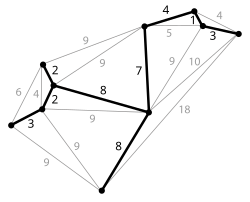
\includegraphics[width=0.7\linewidth]{images/mst_exemple.png}
\end{center}

\end{frame}

% ========================
\section{Algorithmes}
% ========================

\begin{frame}{Outils utilisés}

\begin{block}{Générateur aléatoire}
Création de graphes non orientés, pondérés et connexes.
\end{block}

\begin{block}{Algorithmes gloutons}
Sélectionnent un choix local optimal à chaque étape.
\end{block}

\begin{block}{Union-Find}
Détection efficace des cycles dans Kruskal.
\end{block}

\begin{block}{File de priorité}
Permet à Prim de sélectionner l’arête sortante minimale.
\end{block}

\end{frame}

\begin{frame}{Prim}

\begin{center}
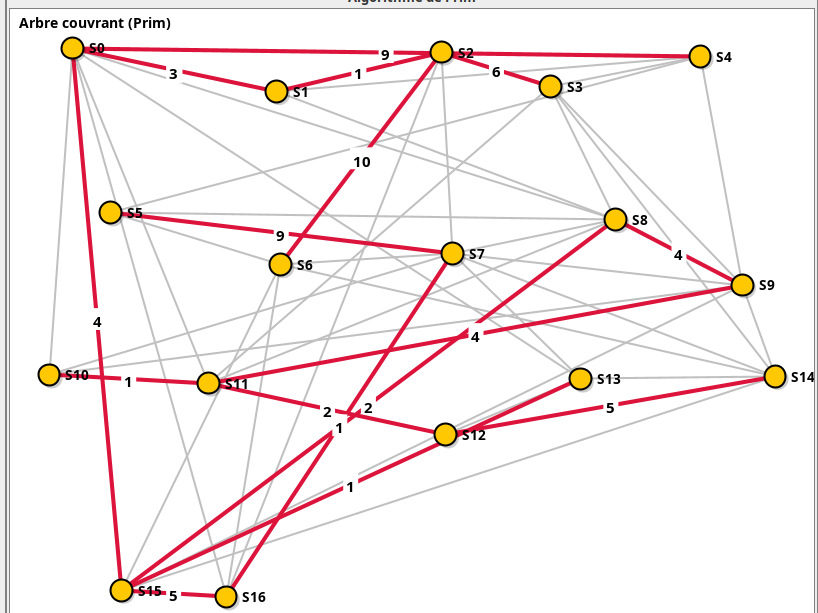
\includegraphics[width=0.45\linewidth]{images/prim_chemin.png}
\end{center}

\begin{itemize}
    \item On part d’un sommet
    \item On ajoute l’arête la plus légère sortant de l’arbre courant
\end{itemize}

\end{frame}

\begin{frame}{Kruskal}

\begin{center}
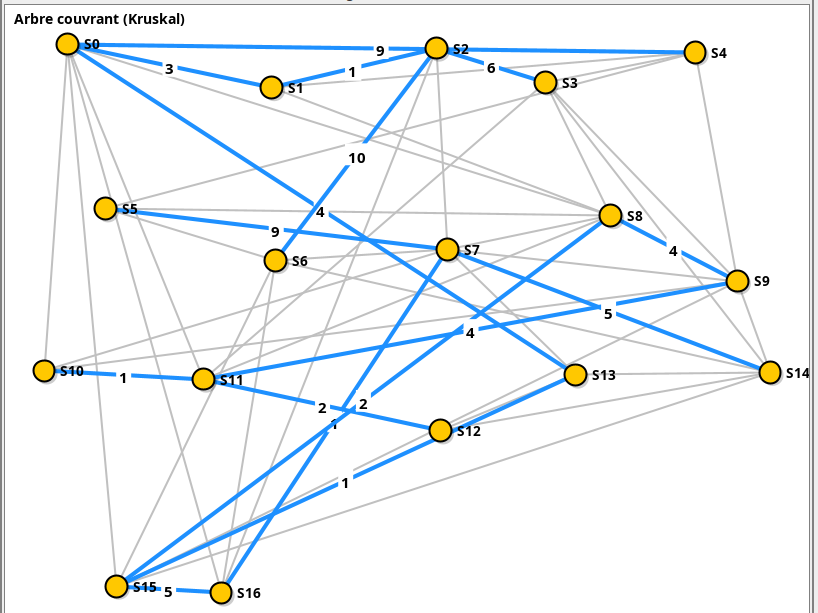
\includegraphics[width=0.45\linewidth]{images/kruskal_tri.png}
\end{center}

\begin{itemize}
    \item Tri des arêtes par poids
    \item Ajout en évitant les cycles (Union-Find)
\end{itemize}

\end{frame}

\begin{frame}{Structure générale}

\begin{columns}
\column{0.5\linewidth}
\textbf{Prim}
\begin{enumerate}
    \item Choisir un sommet de départ
    \item File de priorité (min-heap)
    \item Ajouter l’arête minimale sortante
\end{enumerate}

\column{0.5\linewidth}
\textbf{Kruskal}
\begin{enumerate}
    \item Trier toutes les arêtes
    \item Parcourir de la plus légère à la plus lourde
    \item Ajouter si aucun cycle
\end{enumerate}
\end{columns}

\end{frame}

\begin{frame}{Fonctionnalités du démonstrateur}

\begin{itemize}
    \item Génération aléatoire d’un graphe connexe et pondéré
    \item Exécution \textbf{pas à pas}
    \begin{itemize}
        \item Prim : visualisation de la file de priorité
        \item Kruskal : visualisation du tri des arêtes
    \end{itemize}
    \item Animation de la construction du MST
    \item Résultat final clairement affiché
\end{itemize}

\end{frame}

% ========================
\section{Démonstration}
% ========================

\begin{frame}{Démonstration}
Présentation du démonstraateur.
\end{frame}

% ========================
\section{Comparaison}
% ========================

\begin{frame}{Comparaison : Prim vs Kruskal}

\begin{table}[]
\centering
\begin{tabular}{|c|c|c|}
\hline
\textbf{Critère} & \textbf{Prim} & \textbf{Kruskal} \\ \hline
Point de départ & Un sommet & Aucun \\ \hline
Structure clé & File de priorité & Union-Find \\ \hline
Graphes idéaux & Denses & Clairsemés \\ \hline
Complexité & $O(E\log V)$ & $O(E\log E)$ \\ \hline
Principe & Étend un arbre & Sélectionne les arêtes \\ \hline
\end{tabular}
\end{table}

\end{frame}

% ========================
\section{Conclusion}
% ========================

\begin{frame}{Conclusion}

\begin{itemize}
    \item Les MST permettent d’optimiser divers réseaux.
    \item Prim et Kruskal reposent sur des stratégies gloutonnes efficaces.
    \item Le démonstrateur illustre :
    \begin{itemize}
        \item Le comportement des algorithmes
        \item Les structures de données (tas, Union-Find)
        \item La construction progressive du MST
    \end{itemize}
\end{itemize}

\end{frame}

% ========================
\section{Sources}
% ========================

\begin{frame}{Sources}

\small
\begin{itemize}
    \item Comparaison Prim/Kruskal : \url{https://byjus.com/gate/difference-between-prims-and-kruskal-algorithum/}
    \item Arbre couvrant minimal : \url{https://fr.wikipedia.org/wiki/Arbre_couvrant_de_poids_minimal}
    \item Algorithme glouton : \url{https://fr.wikipedia.org/wiki/Algorithme_glouton}
    \item Algorithme de Prim : \url{https://fr.wikipedia.org/wiki/Algorithme_de_Prim}
    \item Algorithme de Kruskal : \url{https://fr.wikipedia.org/wiki/Algorithme_de_Kruskal}
\end{itemize}

\end{frame}

\end{document}
